

\title{Software Requirements Specification}
\def \documentid {LEANOS-UVIE-SRS-001}
\date{Issue 0.3, June 1, 2017}

\newcommand\affil[1]{\textsuperscript#1}

\def\preparedby {Armin Luntzer\affil{1}}
\def\checkedby {Roland Ottensamer\affil{1}}
\def\approvedby {Franz Kerschbaum\affil{1}}

\def\affiliations{
	\affil{1} Department of Astrophysics, University of Vienna
}




\documentclass{report}
%\usepackage[left = 2cm, right=2cm, top = 1cm]{geometry}
\usepackage[top = 2cm, bottom = 5cm]{geometry}

\usepackage[T1]{fontenc}
\usepackage{textcomp}

%\PassOptionsToPackage{table}{xcolor}


\usepackage{geometry}
\usepackage{fontspec}
%
\defaultfontfeatures[MyriadPro-SemiCondensed]{
	Path		= ../shared/fonts/,
	Extension	= .otf,
	UprightFont	= *-light,
	ItalicFont	= *-italic,
	BoldFont	= *-bold,
	BoldItalicFont	= *-bold-italic
%	LetterSpace	= 5pt		% Laufweite
}
%
\defaultfontfeatures[MyriadPro]{
	Path		= ../shared/fonts/,
	Extension	= .otf,
	UprightFont	= *-regular,
	ItalicFont	= *-italic,
	BoldFont	= *-bold,
	BoldItalicFont	= *-bold-italic
}%
\defaultfontfeatures[MyriadProLight]{
	Path		= ../shared/fonts/,
	Extension	= .otf,
	UprightFont	= MyriadPro-light,
	ItalicFont	= MyriadPro-light-italic,
}

\setmainfont{MyriadPro}



\makeatletter
\renewcommand\normalsize{%
\@setfontsize\normalsize{11pt}{14pt}
\abovedisplayskip 10\p@ \@plus2\p@ \@minus5\p@%
\abovedisplayshortskip \z@ \@plus2\p@%
\belowdisplayshortskip 5\p@ \@plus2\p@ \@minus3\p@%
\belowdisplayskip \abovedisplayskip%
\let\@listi\@listI%
}
\normalsize  
\makeatother



\usepackage{titlesec}

\titleformat{\chapter}[hang]
  {\fontspec{MyriadProLight}\fontsize{30}{36}\selectfont\color{uvie-blue}}
  {\fontspec{MyriadPro}\selectfont\thechapter.}{8pt}{}
\titlespacing*{\chapter}{0pt}{-20pt}{20pt}

\titleformat{\section}
  {\fontspec{MyriadPro}\fontsize{13}{16}\selectfont\color{uvie-blue}}
  {\thesection}{1em}{}

\titleformat{\subsection}
  {\fontspec{MyriadPro}\fontsize{13}{16}\selectfont\color{uvie-blue}}
  {\thesection}{1em}{}

\DeclareMathSizes{12}{55}{15}{15}

\usepackage[table]{xcolor}

% begin UVIE primary colours
\iffalse

% colours from numeric colour values in corporate design document
\definecolor{uvie-blue}{RGB}{0, 99, 166}
\definecolor{uvie-orangered}{RGB}{221, 72, 20}
\definecolor{uvie-goldenyellow}{RGB}{234, 171, 0}
% UVIE secondary colours
\definecolor{uvie-gray}{RGB}{102, 102, 102}
\definecolor{uvie-burgundy}{RGB}{167, 28, 73}

\else
% colours from actual colour samples in corporate design document
%r: 0 g:58 b:133
\definecolor{uvie-blue}{RGB}{0, 79, 150}
\definecolor{uvie-orangered}{RGB}{225, 55, 15}
\definecolor{uvie-goldenyellow}{RGB}{248, 169, 0}
% UVIE secondary colours
\definecolor{uvie-gray}{RGB}{104, 104, 104}
\definecolor{uvie-burgundy}{RGB}{141, 22, 51}

\fi
% end UVIE primary colours


% allowed UVIE logo height
\newlength{\maxlogoheight}\setlength{\maxlogoheight}{20mm}
\newlength{\medlogoheight}\setlength{\medlogoheight}{15mm}
\newlength{\minlogoheight}\setlength{\minlogoheight}{10mm}
%
% allowed space round logo: logoheight <= x <= 0.5 logoheight 
\def \maxlogospacing{1.0}
\def \medlogospacing{0.75}
\def \minlogospacing{0.5}

%
%elif \paperheight \equal {210mm} % A5
% todo: based on papersize: >= A4: 20mm, A5/long: 15mm, all smaller: 10mm
%\if \paperheight \equal {297mm}	  % A4
\newlength{\logoheight}{\setlength{\logoheight}{\maxlogoheight}
%elif \paperheight \equal {210mm} % A5
%\fi
%
% todo: pass as option
\newlength{\logospacing}{\setlength{\logospacing}{\medlogospacing\logoheight}


\newcommand{\fig}[1]{Figure \ref{#1}}


\newenvironment{keywords}%
   {\begin{trivlist}\item[]{\bfseries\sffamily Schlagworte:}\ }% oder "Keywords:"
   {\end{trivlist}}
%
\author{%
    Author 1 name \\
    Department name \\
    \texttt{email1@example.com}\vspace{40pt} \\
    Author 2 name \\
    Department name \\
    \texttt{email2@example.com}
    }


\usepackage{tabu}
\usepackage{colortbl}

\usepackage{array, ltxtable}
\usepackage[most]{tcolorbox}


\usepackage[some]{background}
\usepackage{tikz}
\backgroundsetup{
scale=1,
angle=0,
opacity=1,
placement=top,
contents={
	\begin{tikzpicture}[remember picture, blend mode = multiply]
		% field heights from top down: x | x | x/2 | remainder
		%
		\fill[white]		(-0.5\paperwidth,                 0.0)
							rectangle (0.5\paperwidth,       -3.0\logospacing);
		\fill[uvie-blue!75]	(-0.5\paperwidth,                -3.0\logospacing)
							rectangle (0.5\paperwidth, -2.0 * 3.0\logospacing);
		\fill[uvie-blue]	(-0.5\paperwidth,          -2.0 * 3.0\logospacing)
							rectangle (0.5\paperwidth, -2.5 * 3.0\logospacing);
		% mext can be image or colour, but must overlap with 3rd bar in multiply
		% blend mode
		% todo: make conditional on image option
		\fill[uvie-blue!75]	(-0.5\paperwidth,          -2.0 * 3.0\logospacing)
							rectangle (0.5\paperwidth,       -1.0\paperheight);
	\end{tikzpicture}}
}
%


\makeatletter
\let\doctitle\@title
\makeatother

\makeatletter
\let\docdatever\@date
\makeatother

\usepackage{fancyhdr}
\usepackage{lastpage}

\def\ifalogo{
\includegraphics[height = \medlogoheight]{../shared/images/uni_logo_astrophysik_cmyk.eps}}
\fancypagestyle{plain}{ % call style plain so it is used by chapter pages as well
	\fancyhf{}
	\fancyhead[R]{
		\fontspec{MyriadPro}\docdatever \\
		\vspace{2em}
		Page \thepage\ of \pageref*{LastPage} 
	}

	\fancyhead[C]{
		{
			\fontspec{MyriadPro}
			\documentid \\
			\vspace{.7em}
			\doctitle
			\vspace{.9em}
		}
	}
	\fancyhead[L]{
		\ifalogo%
	}
}
\setlength\headheight{80pt}
\pagestyle{plain}


% def \preparedby, \checkedby, \approvedby, \documentid, \docdatever, \doctitle
\def\approvalpage{
	\clearpage
	\pagestyle{empty}
	\null
	\vfil

	{\fontspec{MyriadPro}\fontsize{20}{24}\selectfont\color{uvie-blue}
	 \doctitle}

	\vspace*{1\baselineskip}

	\begin{tabular}{@{}ll}
		\textbf{Reference:}   & \documentid \\[2ex]
		\textbf{Version:}     & \docdatever \\[6ex]
		\textbf{Prepared by:} & \preparedby \\[1ex]
		\textbf{Checked by:}  & \checkedby  \\[1ex]
		\textbf{Approved by:} & \approvedby \\[1ex]
	\end{tabular}

	\vspace*{0.5\baselineskip}
	{\footnotesize \affiliations}


	\vfill

	\begin{minipage}[b]{0.9\textwidth}
	\footnotesize\raggedright
	\setlength{\parskip}{0.5\baselineskip}
	Copyright \copyright \the\year\ \par
	Permission is granted to copy, distribute and\slash or modify this
	document under the terms of the GNU Free Documentation License,
	Version 1.3 or any later version published by the Free Software
	Foundation; with no Front-Cover, no Logos of the University of Vienna.
	\end{minipage}
	\vspace*{2\baselineskip}
	\cleardoublepage

	\pagestyle{plain}
}

\newcommand{\uvietitlepage}[3]{%
\begin{titlepage}
\BgThispage
%
%
\begin{tikzpicture}[overlay, remember picture]
\node[anchor	= north west,
      xshift	= \logospacing,
      yshift	=-\logospacing] 
      at (current page.north west)
     {
\includegraphics[height = \logoheight]{../shared/images/uni_logo_astrophysik_cmyk.eps}}; 
\end{tikzpicture}
%
\begin{tikzpicture}[overlay, remember picture]
\node[anchor	= north east,
      xshift	=-\logospacing,
      yshift	=-\logospacing] 
      at (current page.north east)
     {
\includegraphics[height = \logoheight]{../shared/images/uni_logo_farbe_02.eps}}; 
\end{tikzpicture}
%
%
%
% main title, must not exceed 3 lines 
\begin{tikzpicture}[overlay, remember picture]
\node[anchor			= north west,
      xshift			= \logospacing,
      yshift			=-\logospacing * 3.0,
	  minimum height	= \logospacing * 3.0,
	  text width		= \textwidth]
      at (current page.north west)
      {\fontsize{30pt}{36pt}\selectfont
       \textcolor{white}
       {
			\uppercase{#1}
       }
       \par
      };
\end{tikzpicture}
%
% subtitle, must not exceed 3 lines 
\begin{tikzpicture}[overlay, remember picture]
\node[anchor			= north west,
      xshift			= \logospacing,
      yshift			=-\logospacing * 5.5,
	  minimum height	= \logospacing * 2.5,
	  text width		= \textwidth]
      at (current page.north west)
      {\fontsize{13pt}{16pt}\selectfont
       \textcolor{white}
       {
			\uppercase{\textbf {#2}}
       }
       \par
      };
\end{tikzpicture}
%
%\noindent
%\hfill
% \hspace*{-3cm}
\begin{tikzpicture}[overlay, remember picture]
\node[anchor=south east,		%anchor is upper left corner of the graphic
      xshift  = 0.5cm,		%shifting around
      yshift  = -0.5cm] 
     	at (current page.south east) %left upper corner of the page
     {\includegraphics[width=14.0cm]{#3}}; 
\end{tikzpicture}
%
%
\end{titlepage}
%
\restoregeometry
%
\newpage
}% newcommand uvietitlepage


\usepackage{xintexpr, xinttools}

\usepackage{xr-hyper} % load before hyperref
\usepackage{hyperref}% check if ok with hyperlinks
\hypersetup{colorlinks=true, linkcolor=uvie-blue}

\usepackage{xifthen}
\usepackage{pifont}
\usepackage{adjustbox}	% \rot

\usepackage{stringstrings}


\newcommand{\requirements}{}
\newcommand{\designs}{}
\providecommand*\phantomsection{}

\makeatletter

\newcommand{\req}[1]{%
	\textbf{R-#1}%
	\phantomsection
	\def\@currentlabel{R-#1}%
	\label{req@#1}%
  	\@ifundefined {req@#1} {%
  		\global\@namedef{req@#1}{}%
  		\g@addto@macro\requirements{{req@#1}}%
	}{}%
}

\newcommand{\reqgoal}[1]{%
	\textbf{G-#1}%
	\phantomsection
	\def\@currentlabel{G-#1}%
	\label{req@#1}%
	\@ifundefined {req@#1} {%
		\global\@namedef{req@#1}{}%
		\g@addto@macro\requirements{{req@#1}}%
	}{}%
}

\newcommand{\meetsthisreq}[1]{% (renamed from \meetsreq above)
  \@ifundefined {req@#1@ismetby} {%
  \global\@namedef{req@#1@ismetby}{}%
  }{}% this is called multiple times when creating a table, generate only one
  \ref{REQ-req@#1}%
  \expandafter\g@addto@macro\csname req@#1@ismetby\expandafter\endcsname 
              \expandafter {\expandafter{\@currentdesign}}%
}

\newcommand{\meetsreq}[1]{% (handles comma separated list)
  \xintListWithSep{, }{\xintApply{ \meetsthisreq}{\xintCSVtoList{#1}}}%
}



\newcommand{\designswithreq}[1]% 
% The space before \ref below is intentional and will be swallowed by \xintApply
% It is not mandatory however, the thing works without it too.
 {\csname #1@ismetby\endcsname}

\newcommand{\designswithreqref}[1]% 
% The space before \ref below is intentional and will be swallowed by \xintApply
% It is not mandatory however, the thing works without it too.
 {\xintListWithSep{, }{\xintApply { \ref}{\csname #1@ismetby\endcsname }}}

\newcommand{\newdesign}[1]{%
  	\textbf{D-#1}%
  	\phantomsection
  	\def\@currentlabel{D-#1}%
	\label{design@#1}%
  	\@ifundefined {design@#1} {%
  		\global\@namedef{design@#1}{}%
		\gdef\@currentdesign{design@#1}%
  	\g@addto@macro\designs{{design@#1}}%
	}{}
}


\newcommand{\design}[5]{%
	\rowcolors{1}{white}{white}%
	\begin{tcolorbox}[enhanced, notitle, clip upper,%
			  sharp corners, colframe = white, colback = white,%
		tabularx={%
						  p{0.15\columnwidth}%
				>{\arraybackslash\raggedright}p{0.10\columnwidth}%
				>{\arraybackslash}X%
			}%
		]%
	%
	\vspace{-.65\baselineskip}	% uuuaaahhh..why? :(
	\cellcolor{uvie-blue!75}\color{white}\newdesign{#1} &%
	\vspace{-.65\baselineskip}%
	\cellcolor{uvie-blue!50}\color{white}\textbf{Identifier} &%
	\vspace{-.65\baselineskip}%
	\cellcolor{uvie-blue!50}\color{white}\textbf{Function} \\%
	& #2 & #3%

	\\%
	\vspace{-1em}%
	\arrayrulecolor{uvie-blue!75}\renewcommand{\arraystretch}{1.2}
	\color{uvie-blue!75}\textbf{Purpose} &%
	\multicolumn{2}{|>{\arraybackslash\raggedright}X}{#4}%

	\ifthenelse{\isempty{#5}} {}{%
		\\%
		\vspace{-1em}%
		\arrayrulecolor{uvie-blue!75}\renewcommand{\arraystretch}{1.2}
		\color{uvie-blue!75}\textbf{Comment} &%
		\multicolumn{2}{|>{\arraybackslash}X}{#5}%
	}%
	\vspace{1em}
	\end{tcolorbox}%
}





\newcommand{\requirement}[4]{%
	\rowcolors{1}{white}{white}%
	\begin{tcolorbox}[enhanced, notitle, clip upper,%
			  sharp corners, colframe = white, colback = white,%
		tabularx={%
						  p{0.15\columnwidth}%
				>{\arraybackslash\raggedright}p{0.15\columnwidth}%
				>{\arraybackslash}X%
			}%
		]%
	%
	\vspace{-.65\baselineskip}	% uuuaaahhh..why? :(
	\cellcolor{uvie-blue!75}\color{white}\req{#1} &%
	\vspace{-.65\baselineskip}%
	\cellcolor{uvie-blue!50}\color{white}\textbf{Short Text} &%
	\vspace{-.65\baselineskip}%
	\cellcolor{uvie-blue!50}\color{white}\textbf{Software Requirement} \\%
	& #2 & #3%

	\ifthenelse{\isempty{#4}} {}{%
		\\%
		\vspace{-1em}%
		\arrayrulecolor{uvie-blue!75}\renewcommand{\arraystretch}{1.2}%
		\color{uvie-blue!75}\textbf{Comment}&%
		\multicolumn{2}{|>{\arraybackslash}X}{#4}%
	}%
	\vspace{1em}
	\end{tcolorbox}%
}



\newcommand{\goal}[4]{%
	\rowcolors{1}{white}{white}%
	\begin{tcolorbox}[enhanced, notitle, clip upper,%
			  sharp corners, colframe = white, colback = white,%
		tabularx={%
						  p{0.15\columnwidth}%
				>{\arraybackslash}p{0.2\columnwidth}%
				>{\arraybackslash}X%
			}%
		]%
	%
	\vspace{-.65\baselineskip}	% uuuaaahhh..why? :(
	\cellcolor{uvie-gray!75}\color{white}\reqgoal{#1} &%
	\vspace{-.65\baselineskip}%
	\cellcolor{uvie-gray!50}\color{white}\textbf{Short Text} &%
	\vspace{-.65\baselineskip}%
	\cellcolor{uvie-gray!50}\color{white}\textbf{Software Requirement} \\%
	& #2 & #3%
	\ifthenelse{\isempty{#4}} {}{%
		\\%
		\vspace{-1em}%
		\arrayrulecolor{uvie-gray!75}\renewcommand{\arraystretch}{1.2}
		\color{uvie-gray!75}\textbf{Comment} &%
		\multicolumn{2}{|>{\arraybackslash}X}{#4}%
	}%
	\vspace{1em}
	\end{tcolorbox}%
}





\newcommand{\exportrequirements}{%
\AtEndDocument{%
	\newwrite\reqfile
	\immediate\openout\reqfile=requirements.list
	\immediate\write\reqfile{\string\renewcommand{\string\requirements}{\requirements}}
	\immediate\closeout\reqfile
}}%


\makeatletter


\newcommand*\traceabilitymatrix[]{%
%
	\newcommand{\numitems}[1]{{\expandafter\xintLength\expandafter{##1}}}%
	\newcommand*\OK{\ding{51}}%
%
	\newcounter{numdesigns}%
	\setcounter{numdesigns}{\numitems{\designs}}%
	\stepcounter{numdesigns}%
%
	\newcommand*\rot{\multicolumn{1}{R{90}{0em}}}%
%
	%\begin{table}[h]
	\newcolumntype{C}{>{\centering\arraybackslash} m{0.2cm}}%
	\newcolumntype{R}[2]{>{\adjustbox{angle=##1,lap=\width-(##2)}\bgroup}l<{\egroup}}%
	\rowcolors{1}{uvie-gray!25}{white}%
	\begin{longtable}{c*{\value{numdesigns}}CC} %+1 linespacing column
	\xintFor* ##1 in \designs \do {%
		&  \rot{\fontspec{MyriadPro}\fontsize{8}{9}\ref{##1}\,\,\normalfont}%
	} \\%
	\endhead
	% it's hilariously inefficient, faster methods are welcome...
	\xintFor* ##1 in \requirements \do {%
	% TODO: recolor link if goal
	%	\isnextbyte[q]{R}{\string\ref{##1}} \par
	%	\if T\theresult moopp\hypersetup{filecolor=uvie-burgundy}\fi

		\fontspec{MyriadPro}\fontsize{8}{9}\ref{REQ-##1}\normalfont %
		\hypersetup{filecolor=uvie-blue}
		\xintFor* ##2 in \designs \do {%
			&%
			\xintFor* ##3 in {\designswithreq{##1}} \do {%
				\ifthenelse{\equal{##2}{##3}} {%
					\cellcolor{uvie-blue!50}%
					%\OK
					\xintBreakFor%
				}{}%
			}%
		}\\[0.1cm]%
	}%
	\end{longtable}%
	%\end{table}%
}%


\usepackage{stringstrings}

\def\rereadauxdesignlabels{
	\newtoks\designlist%
	\newread\zz%
	\immediate\openin\zz=\jobname.aux%
	\loop%
	\ifeof\zz\else%
	\read\zz to \tmp%
	\expandafter\findlabeldesign\tmp\relax\findlabel%
	\repeat%
}


\long\def\findlabeldesign#1#2\findlabel{%
 \ifx\newlabel#1\designlist\expandafter{\the\designlist\showlabeldesign#2}\fi}


%hyperref has 4 felds in each label could use them but don't here
\def\showlabeldesign#1#2{%
	%\begin{minipage}{\textwidth}%
	\findwords[q]{\expandafter\string\detokenize{#1}}{design}%
		\ifnum\theresult>0%
		\par\noindent\ref{#1}\dotfill\pageref{#1}%
		\fi%
	%\end{minipage}%
}


\def\rereadauxrequirementlabels{
	\newtoks\requirementlist
	\newread\zz
	\immediate\openin\zz=\jobname.aux
	\loop
	\ifeof\zz\else
	\read\zz to \tmp
	\expandafter\findlabelrequirement\tmp\relax\findlabel
	\repeat
}


\long\def\findlabelrequirement#1#2\findlabel{%
 \ifx\newlabel#1\requirementlist\expandafter{\the\requirementlist\showlabelrequirement#2}\fi}

\newsavebox{\fminipagebox}
\NewDocumentEnvironment{fminipage}{m O{\fboxsep}}
 {\par\kern#2\noindent\begin{lrbox}{\fminipagebox}
  \begin{minipage}{#1}\ignorespaces}
 {\end{minipage}\end{lrbox}%
  \makebox[#1]{%
    \kern\dimexpr-\fboxsep-\fboxrule\relax
    \fbox{\usebox{\fminipagebox}}%
    \kern\dimexpr-\fboxsep-\fboxrule\relax
  }\par\kern#2
 }


%hyperref has 4 felds in each label could use them but don't here
\def\showlabelrequirement#1#2{%
	\begin{minipage}{\textwidth}%
	\findwords[q]{\expandafter\string\detokenize{#1}}{req}%
		\ifnum\theresult>0%
		\par\noindent\ref{#1}\dotfill\pageref{#1}%
		\fi%
	\end{minipage}%
}

\usepackage[xindy, nopostdot, numberedsection, style=super, section, toc, acronyms, nogroupskip]{glossaries}
\usepackage{xparse}

\setlength{\glsdescwidth}{0.8\textwidth}
\renewcommand{\glsnamefont}[1]{\textbf{#1}}

% label, acronym, name, description
\DeclareDocumentCommand{\newdualentry}{ m m m m } {
	\newglossaryentry{gls-#1}{
	name={#3 (\gls{#1})},
	description={#4}, nonumberlist
	}
	\newglossaryentry{#1}{
		type=\acronymtype,
		name={#2},
		first={#3 (#2)},
		firstplural={#3s (#2s)},
		see={[Glossary:]{\gls{gls-#1}}},
		description=\glslink{gls-#1}{#3},
		nonumberlist
	}%
}
%%% \gls{ABBREV} to point at Acronym/Abbreviation index
%%% \gls{gls-ABBREV} to point to glossary


\newdualentry{ADC}%
  {ADC}%
  {Analog to Digital Converter}%
  {An Analog to Digital Converter is a system that converts an analog signal
   into a quantized digital signal. Its counterpart is the \gls{DAC}.}%

\newdualentry{API}%
  {API}%
  {Application Programming Interface}%
  {The Application Programming Interface defines how a developer can write
   a program that requests services from an operating system or application.
   \glspl{API} are implemented by function calls composed of verbs and nouns,
   i.e. a function to execute on an object.}%

\newdualentry{BSP}%
  {BSP}%
  {Board Support Package}%
  {A Board Support Package is the implementation of a specific interface defined
   by the abstract layer of an operating system that enables the latter to run
   on the particular hardware platform.}%

\newdualentry{CPU}%
  {CPU}%
  {Central Processing Unit}%
  {The Central Processing Unit is the electronic circuitry that interprets
  instructions of a computer program and performs control logic, arithmetic,
  and input/output operations specified by the instructions. It maintains
  high-level control of peripheral components, such as memory and other devices.}%

\newdualentry{DAC}%
  {DAC}%
  {Digital to Analog Converter}%
  {A Digital to Analog Converter is a system that converts a quantized digital
   signal into an analog signal. Its counterpart is the \gls{ADC}.}%

\newdualentry{DMA}%
  {DMA}%
  {Direct Memory Access}%
  {Direct Memory Access is a feature of a computer system that allows hardware
   subsystems to access main system \gls{gls-RAM} directly, thereby bypassing
   the \gls{gls-CPU}.}%

\newdualentry{DSP}%
  {DSP}%
  {Digital Signal Processor}%
  {A Digital Signal Processor is a specialised processor with its architecture %
   targeting the operational needs of digital signal processing.}%

\newdualentry{ELF}%
  {ELF}%
  {Executable and Linkable Format}%
  {The Executable and Linkable Format is a common standard file format for
   executables, object code, shared libraries, and core dumps.}%

\newdualentry{FIFO}%
  {FIFO}%
  {First In - First Out}%
  {In FIFO processing, the "head" element of a queue is processed first.
   Once complete, the element is removed and the next element in line becomes
   the new queue head.}%

\newdualentry{FPU}%
  {FPU}%
  {Floating Point Unit}%
  {A co-processor unit that specialises in floating-point calculations.}%

\newdualentry{ILP}%
  {ILP}%
  {Instruction Level Parallelism}%
  {Instruction-level parallelism (ILP) is a measure of how many instructions in
   a computer program can be executed simultaneously by the \gls{CPU}.}%

\newdualentry{ISR}%
  {ISR}%
  {Interrupt Service Routine}%
  {An Interrupt Service Routine is a function that handles the actions needed
   to service an interrupt.}%

\newdualentry{GCC}%
  {GCC}%
  {GNU Compiler Collection}%
  {The GNU Compiler Collection is a compiler system produced by the
   GNU project. It is part of the GNU toolchain collection of programming
   tools.}%

\newglossaryentry{GNU}{
  name={GNU},
  description={GNU is a recursive acronym that stands for "GNU's Not Unix!".
	      The GNU project is a free software collaboration project announced
	      in 1987. Users are free to run GNU-licensed software, share, copy,
	      distribute, study and modify it. GNU software guarantees these
	      freedom-rights legally via its license and is thefore free
      	      software.},
  nonumberlist
}

\newglossaryentry{LEON2}{
  name={LEON2},
  description={The LEON2 is a synthesisable VHDL model of a 32-bit processor
	       compliant with the SPARC V8 architecture. It is highly
	       configurable and particularly suitable for \gls{SoC} designs.
	       Its source code is available under the GNU LGPL license},
  nonumberlist
  }

\newglossaryentry{LEON3}{
  name={LEON3},
  description={The LEON3 is an updated version of the \gls{LEON2}, changes
	       include \gls{gls-SMP} support and a deeper instruction pipeline},
  nonumberlist
  }

\newglossaryentry{LEON3-FT}{
  name={LEON3-FT},
  description={The LEON3-FT is a fault-tolerant version of the \gls{LEON3}.
  	       Changes to the base version include autonomous error handling,
       	       cache locking and different cache replacement strategies.},
  nonumberlist
  }

\newdualentry{MMU}%
  {MMU}%
  {Memory Management Unit}%
  {A Memory Management Unit performs address space translation between physical
   and virtual memory pages and protects unprivileged access to certain memory
   regions.}%

\newdualentry{MPPB}%
  {MPPB}%
  {Massively Parallel Processor Breadboarding system}%
  {The Massively Parallel Processor Breadboarding system is a proof-of-concept %
   design for a space-hardened, fault-tolerant multi-DSP system with various %
   subsystems to build a powerful digital signal processing system with a high %
   data throughput. Its distinguishing features are the \gls{gls-NoC} and the
   \gls{Xentium} \glspl{DSP} controlled by a \gls{LEON2} processor.
   It was developed under ESA contract 21986 by Recore Systems B.V.}%

\newdualentry{NGAPP}%
  {NGAPP}%
  {Next Generation Astronomy Processing Platform}%
  {Next Generation Astronomy Processing Platform was an evaluation of the
   \gls{MPPB} performed in a joint effort of RUAG Space Austria and the
   Department of Astrophysics of the University of Vienna.
   The project was funded under ESA contract 40000107815/13/NL/EL/f.}%

\newdualentry{NoC}%
  {NoC}%
  {Network On Chip}%
  {A Network On Chip is a communication system on an integrated circuit that
   applies (packet based) networking to on-chip communication. It offers
   improvements over more conventional bus interconnects and is more scalable
   and power efficient in complex \gls{gls-SoC} desgins.}%

\newdualentry{POSIX}
  {POSIX}
  {Portable Operating System Interface}
  {The Portable Operating System Interface is a family of standards specified
   by the IEEE Computer Society for maintaining compatibility between
   operating systems.}%

\newdualentry{PUS}
  {PUS}
  {Packet Utilisation Standard}
  {The Packet Utilisation Standard addresses the end-to-end transport of telemetry
   and telecommand data between user applications on the ground and applications
   onboard a satellite. See also ECSS-E-70-41A.}%

\newdualentry{RAM}%
  {RAM}%
  {Random-Access Memory}%
  {Random-Access Memory is a type of memory where each memory cell may be
   accessed directly via their memory addresses.}%

\newdualentry{RISC}%
  {RISC}%
  {Reduced Instruction Set Computing}%
  {RISC is a \gls{CPU} design strategy that intends to improve performance by
   combining a simplified instruction set with a microprocessor architecture
   that is capable of executing an instruction in a smaller number of clock
   cycles.}%

\newdualentry{RMAP}%
  {RMAP}%
  {Remote Memory Access Protocol}%
  {The Remote Memory Access Protocol is a form of \gls{SpaceWire} communication
   that transparently communicates writes to memory mapped regions between
   different hardware devices.}%


\newdualentry{RR}%
  {RR}%
  {Round Robin}%
  {Round Robin is a scheduling algorithm where time slices are assigned in equal
   poritions and in circular order. In the context of threads, priorities are
   usually only used to control re-scheduling order when a mutex is accessed by
   a thread.}%

\newacronym{RSA}{RSA}{RUAG Space Austria}

\newdualentry{SMP}%
  {SMP}%
  {Symmetric Multiprocessing}%
  {Symmetric Multiprocessing denotes computer architectures, where two or more
   identical processors are connected to the same periphery and are controlled
   by the same operating system instance.}%

\newdualentry{SoC}%
  {SoC}%
  {System On Chip}%
  {A System On Chip is an integrated circuit that combines all components of a %
   computer or other electronic system into a single chip.}%

\newglossaryentry{SpaceWire}{
  name={SpaceWire},
  description={SpaceWire is a spacecraft communication network based in part
               on the IEEE 1355 standard of communications.},
  nonumberlist
  }

\newglossaryentry{SPARC}{
  name={SPARC},
  description={SPARC ("scalable processor architecture") is a \gls{gls-RISC}
  	       instruction set architecture developed by Sun Microsystems in
	       the 1980s. The distinct feature of SPARC processors is the high
	       number of \gls{gls-CPU} registers that are accessed similarly to
	       stack variables via ``sliding windows''.},
  nonumberlist
  }

\newdualentry{SSDP} % label
  {SSDP}            % abbreviation
  {Scalable Sensor Data Processor}  % long form
  {The Scalable Sensor Data Processor (SSDP) is a next generation on-board %
   data processing mixed-signal ASIC, envisaged to be used in future scientific %
   payloads requiring high-performance on-board processing capabilities. %
   It is built opon a heterogeneous multicore architecture, combining two %
   \gls{Xentium} \gls{DSP} cores with a general-purpose \gls{LEON3-FT} control %
   processor in a \gls{gls-NoC}.} % description


\newdualentry{TCM}%
  {TCM}%
  {Tightly-Coupled Memory}%
  {Tightly-Coupled Memory is the local data memory that is directly accessible %
   by a Xentium's load/store unit. It can be viewed as a completely %
   program-controlled data cache.}%


\newacronym{UVIE}{UVIE}{University of Vienna}

\newdualentry{VLIW}%
  {VLIW}%
  {Very Long Instruction Word}%
  {Very Long Instruction Word is a processor architecture design concept that
   exploits \gls{gls-ILP}. This approach allows higher performance at a smaller
   silicone footprint compared to serialised instruction processors, as no
   instruction re-ordering logic to exploit superscalar capabilities of the
   processor must be integrated on the chip, but requires either code to be
   tuned manually or a very sophisticated compiler to exploit the full potential
   of the processor.}%

\newglossaryentry{Xentium}{
  name={Xentium},
  description={The Xentium is a high performance \gls{gls-VLIW} \gls{DSP} core.
               It operates 10 parallel execution slots supporting 32/40 bit
	       scalar and two 16-bit element vector operations.},
  nonumberlist
  }


% do not remove
\glsresetall
\makeglossaries


\usepackage{vhistory}

\usepackage{biblatex}
\addbibresource{../shared/bibliography.bib}

\rereadauxrequirementlabels

\exportrequirements


\begin{document}


\setmainfont{MyriadPro-SemiCondensed}
\uvietitlepage%
{Lean OS --\\ An operating system for the SSDP}%
{\doctitle}%
{../shared/images/logo2.pdf}
\setmainfont{MyriadPro}

\approvalpage

\tableofcontents
\newpage


\chapter*{List of Requirements}
\the\requirementlist


\begin{versionhistory}
  \vhEntry{0.0}{24.07.2015}{AL}{draft requirements created based on \gls{NGAPP}}
  \vhEntry{0.1}{30.03.2016}{AL}{initial version with specifications from \gls{MPPB}v2}
  \vhEntry{0.2}{11.04.2016}{AL}{revised after internal design review}
  \vhEntry{0.3}{01.06.2017}{FK}{document approved}
\end{versionhistory}


\chapter{Introduction}

\section{Purpose of the Document}

This document specifies the software requirements for the operating system
kernel LeanOS. LeanOS targets the \gls{SSDP}, and to a lesser extent, its
compatible predecessor, the \gls{MPPB} v2.x \cite{MPPB}.
It is intended to be used in unmanned space applications of at least
Software Criticality Level C. Readers must be familiar with the basic concepts
of event driven real time operating systems and the target hardware. \\

\noindent
This document follows the document structure for software requirement
specifications found in Annex D of ECSS-E-ST-40C \cite{ECSS40C}.

\section{Scope of the Software}

LeanOS is a lightweight operating system targeting the particular
characteristics of the \gls{SSDP} and is focused on driving the \gls{NoC} and
its attached \gls{Xentium} \gls{DSP} cores.

\chapter{Applicable and Reference Documents} % does not break automatically for some reason

\printbibliography[heading=none]


\chapter{Terms, Definitions and Abbreviated Items}
\printglossary[type=acronym]
\printglossary[type=main, style=altlist]



\chapter{Software Overview}

\section{Function and Purpose}

In the course of the \gls{NGAPP} activities, an evaluation of the \gls{MPPB}
was performed in a joint effort of \gls{RSA} and the Department of Astrophysics
of the \gls{UVIE}. While the original intent of the work of \gls{UVIE} was to
quantify the performance of the \gls{Xentium} \glspl{DSP} and the \gls{MPPB} as a
whole with regard to on-board data treatment and reduction in an astronomical
mission setting, it was found that, given the highly innovative nature of this new
processing platform, a novel approach was needed concerning the management of
system resources, \gls{DMA} mechanics and \gls{DSP} program design for best
efficiency and turnover rates. Consequently, \gls{UVIE} developed an experimental
operating system to stably drive the \gls{DSP} cores and the \gls{MPPB} close
to its performance limit. LeanOS is a development based on this operating system
concept. Along with its intended functionality, it provides full software test
coverage, example applications and good documentation that supports all aspects
of the software.


\section{Environmental considerations}

LeanOS is only required to support the \gls{SSDP}, but will also support the
\gls{MPPB} v2.x. Ultimately, this does allow reuse of the operating system core
for \gls{LEON2} and \gls{LEON3} based platforms with minor adaptations.
Even though the \gls{SSDP} does not contain multi-core \gls{LEON3} processor,
\gls{SMP} support will be prepared in LeanOS, as this will likely change with
newer versions of the \gls{SSDP}.
LeanOS is released under an open source license, so compatible development tools should
be available under such licenses as well. Note that it might still be necessary
to use a commercial product to target particular configurations or proprietary
hardware functionality.


\section{Relation to other systems}

LeanOS is a stand-alone software product.


\section{Constraints}

LeanOS primarily targets the \gls{SSDP}, which effectively limits the hardware
support the the characteristics of this platform. \\
\noindent
The source code is written in C and if required, \gls{SPARC} v8 compatible
assembly. This is necessary as hardware interaction of a machine level requires
programming languages designed for that purpose.



\chapter{Requirements}

\section{General}

%\begin{figure}[ht]
%\begin{center}
%	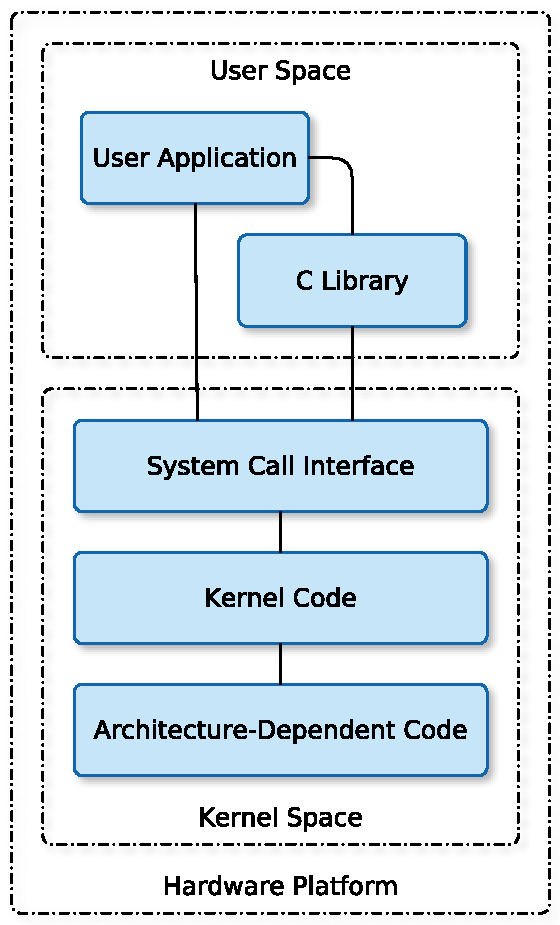
\includegraphics{images/OS_fundamental_architecture}
%	\caption{The fundamental architecture of LeanOS.}
%	%\label{fig:blackbody_curves}
%\end{center}
%\end{figure}

\requirement{GEN-0001} {No external dependecies}{%
LeanOS shall not make use of external libraries, including C-Runtime libraries.
}{}%

\requirement{GEN-0002} {Custom libc functionality}{%
LeanOS shall, as part of its code-base and as needed, provide its own
implementations of typical C-libary functions with an \gls{API} conforming to
their \gls{POSIX} definitions.
}{%
The collection of these functions can also form the base or a subset of a
C-Libary to be used by applications.}%

\requirement{GEN-0003} {Application libc usage}{%
LeanOS shall optionally call a function that initialises a C-Library on startup.
It is up to the user to define and link the implementation of this function and
the according C library.
}{%
The function \_\_libc\_start\_main() is declared as a weak symbol and tested
before execution.
}%


% TODO: to interface requirements?
% example:
%
% declare:
% __libc\_start\_main() __attribute__((weak));
%
% optional execution:
%
% if (__libc_start_main())
%	__libc_start_main();
% }
% it is executed if the function is actually defined or linked in:
%
%  int __libc_start_main()
% {
%	...
% }

\requirement{GEN-0004} {Fatal Error Management}{%
If a non-recoverable error state is detected in LeanOS, it shall optionally
call an error handling routine provided by the user before issuing a reboot.
LeanOS shall provide a directive to register such a function.
}{%
This gives the user the possiblity to perform a clean shutdown of critical
tasks in their particular environment.}%


\requirement{GEN-0006} {Core runtime}{%
In its basic configuration, LeanOS shall restrict itself to the initialisation
of its core services on a single processor, thereby configuring traps, memories
and timers. All other services or device drivers shall be configured and added
via the build system.
}{}%

\requirement{GEN-0601} {Error Logging}{%
LeanOS shall maintain an error message log that is readable by the user.
}{}%

\requirement{GEN-0602} {Coding Style}{%
LeanOS code shall use the Linux kernel coding style. Source files and patches
shall be checked using the checkpatch.pl utility found in the Linux kernel
source tree.
}{%
A major point of LeanOS is that it does not only come with an open source
license, but should ideally only use tools that are distributable under a
similar license. The Linux kernel is used in billions of devices word-wide,
its coding style is hence arguably well-suited for use in successful software.
}%


\section{Functional Requirements}

\requirement{FUN-0007} {SMP support}{%
LeanOS shall be able to run on a multi-core configuration of a LEON3 processor.
}{}%

\requirement{FUN-0803} {MMU support}{%
LeanOS shall support the use of the MMU of the LEON3 processor.
}{}%

\requirement{FUN-0008} {Supervisor Mode}{%
The LeanOS kernel shall execute with the SPARC supervisor mode enabled.
Application code shall run with supervisor mode disabled.
}{}%

\requirement{FUN-0011} {Timing}{%
LeanOS shall provide access to typical time keeping, time taking and delay
timing functionality expected by an operating system.
}{}%


\requirement{FUN-0012} {Task Support}{%
LeanOS shall provide means to create new tasks.
}{}%

\requirement{FUN-0013} {Task priorites and deadlines}{%
LeanOS shall support the assignment of a priority and a deadline to a task.
}{}%

\requirement{FUN-0014} {Task scheduling}{%
LeanOS shall offer a fixed priority scheduler with priority inversion handling.
}{}%

\goal{FUN-0015} {Other schedulers}{%
LeanOS should offer an Earliest Deadline First scheduler supporting priority
execution in overload conditions.
}{%
Along with dynamic ticking, this is an option to optimise thread CPU utilisation
with the added benefit of predictable execution for certain high-priority
threads in conditions where the total load unexpectedly would exceed 100\%.
}%

\requirement{FUN-0016} {Kernel Ticks}{%
LeanOS shall operate in tickless (non-periodic) timed wakeup mode by default.
}{%
Tickless timing avoids unnecessary wake-ups of the CPU if no task is running
and improves performance by only switching to kernel mode from regular tasks
when absolutely necessary.
}%

\requirement{FUN-0017} {Tickless Timing}{%
LeanOS timing functionality shall be able to operate in tickless mode, where 
a queue of wakeup times is maintained and a hardware timer is used in such a way
that its next underflow (resulting in an interrupt) is programmed to coincide
with the next wakeup time. New wakeup times shall be inserted into the queue as
needed to maintain the desired timeline of events and the hardware timer
be readjusted accordingly.
}{}%

\requirement{FUN-0019} {Semaphores and Mutexes}{%
LeanOS shall provide semaphores and mutexes as part of its task functionality.
Task priorities shall be protected by the priority ceiling protocol.
}{}%

\requirement{FUN-0020} {Tasks and \gls{SMP}}{%
LeanOS shall support task migration between \glspl{CPU} and track and ensure
atomicity of related functions (e.g. mutexes) across multiple processors.
}{}%

\requirement{FUN-0021} {Message Queues}{%
LeanOS shall support message queues for inter-process communication.
Atomicity of queues shall be ensured across multiple processors.
}{}%

\requirement{FUN-0022} {Kernel Modules}{%
LeanOS shall offer loadable module support infrastructure.
}{}%

\requirement{FUN-0804} {Kernel-Userspace Initialisation}{%
LeanOS shall offer a configurable initialisation point that executes a
user-space setup procedure.
}{This is the point where the application software is loaded.}%

\requirement{FUN-0023} {System Control Interface}{%
LeanOS shall offer a way for drivers or other functional modules to export
configuration or state variables into an logical tree maintained by
the operating system. This logical tree shall be accessible by other modules and
the user as a character-based interface.
}{%
This is supposed to be a centrally organised, generic parseable interface to
get or set configuration states or system statistics.
}%

\requirement{FUN-0024} {Binary System Control Interface}{%
LeanOS shall offer the possibility to install binary exchange nodes within the
System Control Interface tree that may be used for larger amouts of binary data.
The binary format shall be defined by the creator of the node. Any users of the
node shall be responsible to read or write in the correct format expected by the
node.%
}{%
Sometimes, a binary dump to or from a subsystem is needed that is only parseable
with special knowledge. This could, for example, be an internal memory dump or
some calibration data.
}%

\goal{FUN-0025} {Device Drivers}{%
LeanOS should come with device drivers for all hardware functionality of the SSDP.
}{}%

\requirement{FUN-0026} {Xentium Scheduler}{%
LeanOS shall offer a way to define and load Xentium data processing code.
}{}%

\requirement{FUN-0027} {Xentium Data Buffers}{%
LeanOS shall provide packet-driven meta-data buffers to Xentium programs that
can link to arbitrary data sets and routing tables that define the path of
a data packet through a series of Xentium program nodes.
}{%
Datagrams propagate through processing nodes as defined in their routing table,
which represents their individual ``processing chain''.}%


\section{Performance Requirements}

\requirement{GEN-0009} {Traps/Interrupts}{%
LeanOS trap entry and exit code shall not exceed 500 instructions.
}{%
This does not include the callback functions for a trap or interrupt
service routine.
}%

\requirement{GEN-0018} {Deferred saving of \gls{FPU} registers}{%
In trap mode, LeanOS shall defer saving of \gls{FPU} registers until it is
accessed.
}{%
This approach saves many clock cycles, as the \gls{FPU} is not typically used
as part of an \gls{ISR}.
}%


\requirement{GEN-0010} {Interrupt downtime}{%
\glspl{ISR} that execute longer than 50 µs shall be set to be executed in
deferred mode at a later time if feasible given the type and rate of an \gls{ISR}.
}{
Interrupt mode should be left as fast as possible, so regular processing can
continue. Most \glspl{ISR} requiring long processing times perform actions on
data, which can typically be moved into a dedicated thread, with the \gls{ISR}
acting as a signalling function.
}%

\requirement{GEN-0028} {Real-Time Thread Support}{%
LeanOS shall offer support for a class of real time threads that may also
preempt the operating sytem with the exception of \glspl{ISR}.
}{%
Some application real time tasks may be so timing sensitive, that even
operating system code must be preemptible to guarantee a timely response.
}%

\section{Interface Requirements}

\requirement{GEN-2001} {Interface Documentation}{%
The internal and external interfaces of LeanOS shall be described as part
of its source code in Doxygen markup.
}{
The interfaces of a complex piece of software such as an operating system
often change over time, as it is adapted to new circumstances or improved
implementation of particular functionality or just subtle changes that may not
always propagate into other documents as they should. It is therefore better to
maintain interface documentation together with the code it describes, where it
will be more likely to be updated on the spot.
}%


\section{Operational Requirements}

No operational requirements have been identified.


\section{Resources Requirements}

\requirement{GEN-0101} {Target Platform}{%
LeanOS shall execute on the \gls{SSDP}, in particular the \gls{LEON3-FT}
processor of the platform. It should also execute on the \gls{MPPB} v2.x.
}{}%


\section{Design Requirements and Implementation Constraints}


\requirement{GEN-0801}{Modular Design}{%
All components of LeanOS shall be written such that a particular component does
contain its intended functionality as much as possible.
}{
If something is mostly self-contained, it is easier to modify and re-use in
another software project.
}%

\requirement{GEN-0802}{Software Hierarchy}{%
All components shall make use and rely only on functionality that is lower
in hierarchy. The use of functionality that is hierarchially equal or higher
shall be explicitly forbidden.
}{
Note that hierarchy refers to the abstraction level of a component. An \gls{ISR}
is of higher level than the interrupt dispatcher. Even though it is called by
the latter, the actual registration of the \gls{ISR} is done by a higher level
component. Such constructs are legal, the reliance on user-space provided
functionality, e.g. an error reporting function, which sends messages via some
packet interface on the other hand, is not.
}%


\requirement{GEN-0805}{Programming Language}{%
The programming language shall be C. \gls{SPARC}v8 compatible assembly shall be
used when necessitated by performance or timing constraints and interface
requirements.
}{}%




\section{Security and Privacy Requirements}

No security or privacy requirements have been identified.

\section{Software Quality Requirements}

\goal{GEN-0201} {Product Metrics}{%
LeanOS should have a cyclomatic complexity of at most 15 and a nesting level of
at most 6 per function. Each function shall have a single exit point for the 
nominal case.
}{}%

\section{Software Reliability Requirements}

No software reliability requirements have been identified.

\section{Software Maintainability Requirements}

\requirement{GEN-0301} {Version Identification}{%
It shall be possible to identifiy the version of compiled binary software
components by reading their identifier from a special memory segment.
}{
The build identifier or version number should be set and defined when building
the binary.
}%


\section{Software Safety Requirements}

\requirement{GEN-0401} {Stack Pointer Checks}{%
The stack pointer of a task shall be checked for feasibility before scheduling
the latter.
}{
}%

\requirement{GEN-0402} {Correctable Traps}{%
LeanOS shall provide handlers for correctable traps caused by kernel or user
code and either correctly execute the desired operation (e.g. unaligned access)
or replace the result with a default value (e.g. divison by zero) and skip the
offending code instruction to continue.
}{
}

\requirement{GEN-0403} {Trap Error Reporting}{%
LeanOS shall make an entry into its error message log when a trap event occurs,
describing the nature and source of the trap.
}{
}



\section{Software Configuration and Delivery Requirements}

\requirement{GEN-0005} {Build configuration}{%
LeanOS shall make use of the Linux Kernel Build System (kbuild) for its
configuration.
}{}%


\section{Data Definition and Database Requirements}

No data definition or database requirements have been identified.


\section{Human Factors Related Requirements}

No human factors related requirements have been identified.

\section{Adaptation and Installation Requirements}

No adaptation and installation requirements have been identified.


\chapter{Validation Requirements}

\requirement{GEN-1001} {Verification Method}{%
The verification method and verification activity shall be specified 
in a Software Qualification Test Plan for each requirement.
}{}%

\requirement{GEN-1002} {Qualification Testing}{%
SW qualification testing shall be performed with various configurations of
LeanOS.
}{}%


%\begin{description}
%  \item\design{SRT-0001} First design. \meetsreq{GEN-0001}
%  \item\design{SRT-0002} Second design. \meetsreq{GEN-0001}
%  \begin{description}
%    \item\design{SRT-0002.1} Third design. \meetsreq{GEN-0002}
%    \item\design{SRT-0002.2} Fourth design \meetsreq{GEN-0004, GEN-0005}
%  \end{description}
%\end{description}

%\traceabilitymatrix


\chapter{Traceability}

The requirements in this document are both user and system requirements.
Traces from design and test to the software requirements are given in the
respective documents.


\chapter{Logical Model Description}

\begin{figure}[htb]
\begin{center}
	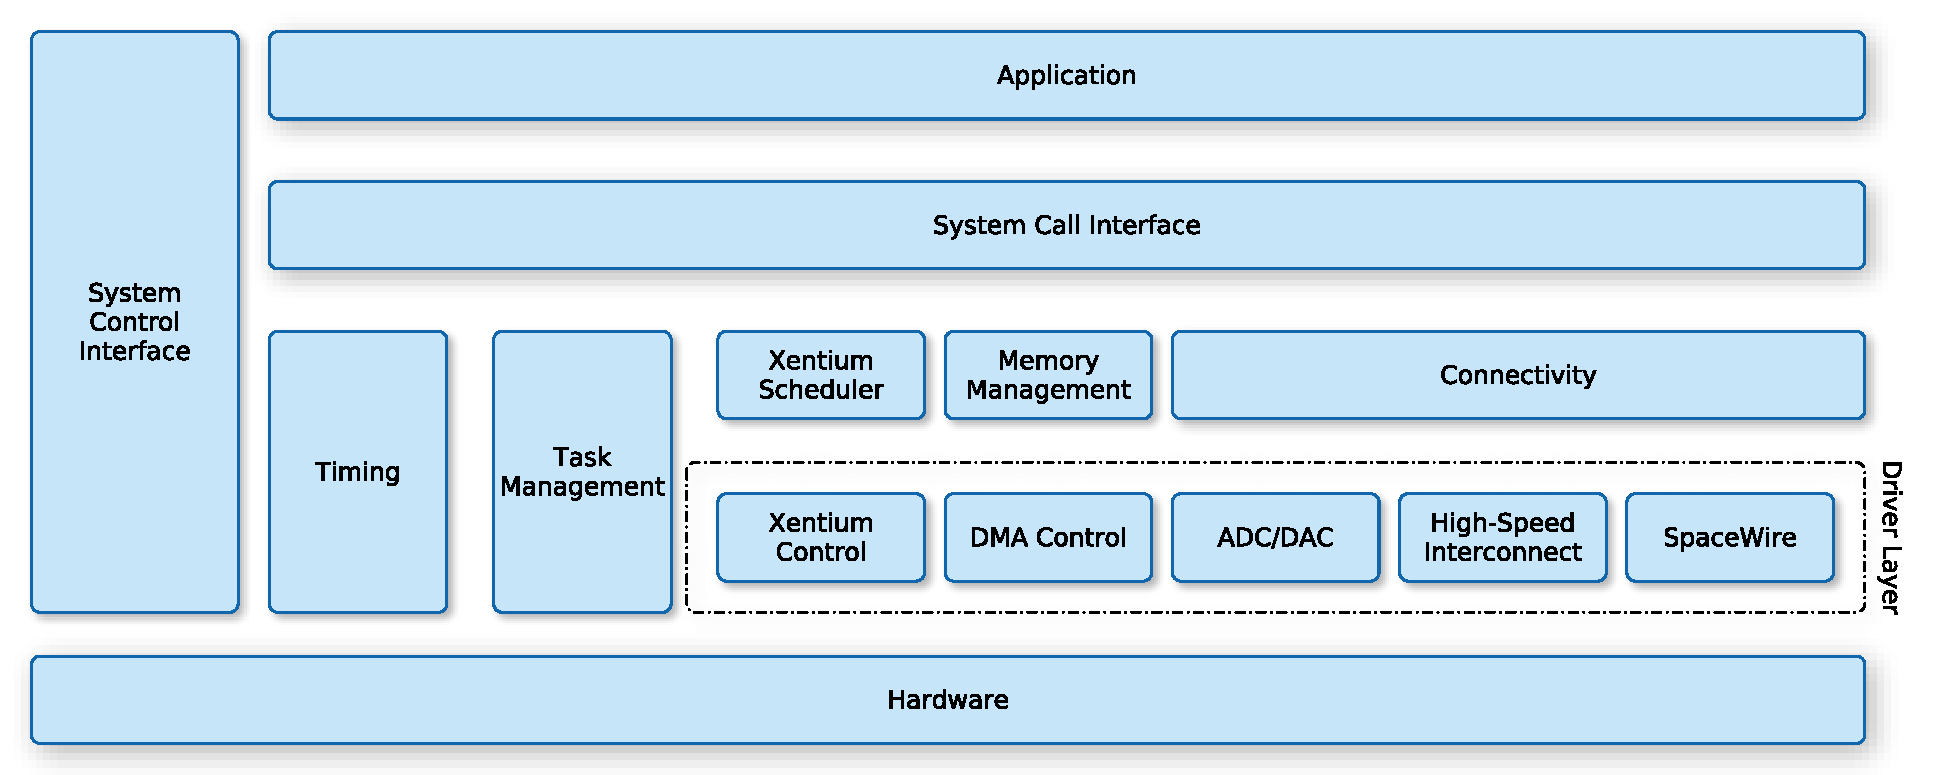
\includegraphics[width=\columnwidth]{images/OS_logical}
	\caption{The logical model of LeanOS. Here, the "hardware" layer
	represents both the hardware and the hardware abstraction layer of
	the software.}
	\label{fig:logical_model}
\end{center}
\end{figure}

In LeanOS, the \gls{SSDP} hardware is accessed in multiple layers of
abstraction (see \fig{fig:logical_model}). Typical \gls{CPU} tasks such as thread/task
management and timer operation are used as part of the operating system kernel
and are also accessible by user applications via a system call interface.
Other functional hardware components of the \gls{SSDP} such as the \gls{NoC}
\gls{DMA} have their own driver modules. These are in turn used by the
\gls{Xentium} scheduler and other higher level modules in the operating system.
Configuration of and access to the latter from user space is done via a system
call interface. The system control interface serves as an intermediate between
all layers of the operating system, where system or module states and hardware
modes or usage statistics may be exported by individual components for external
(user) access.



%\chapter*{Document Change History}


\end{document}
